\begin{appendices}

\chapter{Survey} \label{app:budgetsurvey}
Informal survey of 12 CS students in the third year lab. 

Questions:
\begin{enumerate}
\item Do you currently make a budget?
\item Do you stick to that budget?
\item Do you find your budget has a `positive' impact?
\end{enumerate}

% Booktabs require to add  to your document preamble
\begin{table}[h]
\centering
\caption{Survey Results}
\begin{tabular}{@{}llll@{}}
\toprule
       & \multicolumn{3}{l}{Question} \\ 
Answer & 1.       & 2.      & 3.      \\ \midrule
yes    & 5        & 1       & 3       \\
no     & 7        & 4       & 4       \\
n/a    & 0        & 7       & 5       \\ \bottomrule
\end{tabular}
\end{table}

\begin{comment}
Appendix A, B, C, etc.
These appendices can be very useful for giving detail that would otherwise disrupt the flow and readability of the report. They are given titles (e.g. "Appendix A: Example of the operation of the system") and bound in with the report. In general they are optional though, by convention, for a programming project, Appendix A often contains a non-trivial illustrative example of an input to the system and the corresponding output. For some projects, appendices may include tables of data. However, very long tables of data (more than about 10 pages) should be relegated to the Auxiliary Material, and not submitted as part of the Final Report. Program listings (apart from short code snippets) should likewise not be submitted as part of the Final Report.
\end{comment}

\chapter{Hashing Test} \label{app:hashingtest}

Implemented in PHP, the test was run on a computer with a 2.7 Ghz Intel Core i7, 16Gb of 1600Mhz DDR3 RAM and PHP CLI 5.5.3.

\lstinputlisting[style=phpcolor]{code/passwordHashingTest.php}

\chapter{Database Schema} \label{cha:databaseschema}

\begin{figure}[p]
    \vspace*{-2cm}
    \makebox[\linewidth]{
        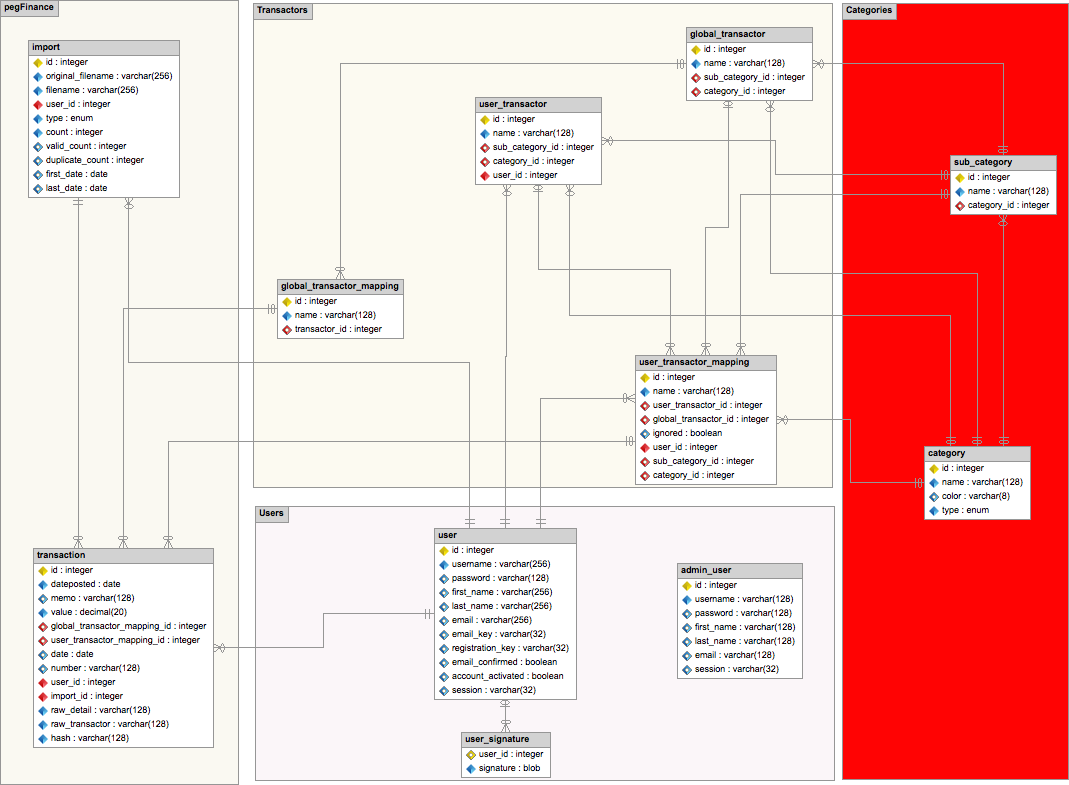
\includegraphics[width=1.3\linewidth,angle=90]{design/database-schema.png}
    }
    \caption{Full database schema for the project}
\end{figure}

\chapter{External Libraries} \label{app:externallibraries}

A full list of libraries and frameworks used by pegFinance are included below, includng licensing information.

\section{Back End}
\subsubsection{pegFramework}
MVC framework that pegFinance is based around. 

Licence - self developed, open-source under the MIT license

\subsubsection{Propel}
ORM library for PHP, that converts schemas based in XML into PHP objects and provides database connectivity.
%
The database objects found within pegFinance are defined in, and generated by Propel. 

License - open-source project released under the MIT license

\subsubsection{Less}
CSS pre-processor that extends the CSS, adding additional features and functionality. `.Less` files compile to `.css`.
%
The CSS for pegFinance is written in and compiled with Less.

License - open-source under the Apache 2 License

\section{Front End}
\subsubsection{jQuery}
A `feature-rich JavaScript library', that provides element selection and enabled HTML traversal and manipulation, as well as providing an easy API for Ajax requests.
%
Used throughout the site for frontend effects, and used heavily in the suggestion wizard.

License - open-source, released under the MIT license

\subsubsection{Bootstrap}
Front-end framework for faster web development that provides a large collection of predefined CSS classes and elements for use on the page.
%
Used for the UI of pegFinance.

License - MIT license and copyright 2014 Twitter

\subsubsection{Inspiritas}
A theme for bootstrap, that defines colors and additional elements for use on the page.
%
A heavily modified version is used for the UI of pegFinance.

Licence - Open-source, Apache License

\subsubsection{StrongPass.js}
jQuery Password Strength plugin for Twitter Bootstrap.
%
Modified version used to provide a client side indication the password entropy calculation during signup.

License - Dual, under the MIT and GPL.

\subsubsection{Pines Notify}
jQuery Pines Notify Plugin. Used to provide event notification in the user interface to indicate events.
%
pNotify is used in the suggestion wizard and when mapping a reference to a transactor to update the user on the status of the request

Licence - Triple licensed under the GPL, LGPL, and MPL.

\subsubsection{UserVoice JavaScript SDK}
SDK for access to a user opinion platform, to help provide insight into the userbase and receive feedback.
%
Deployed throughout the application so users can provide feedback when using the application, including an optional screen capture.

Licence - Commercial SDK provided by UserVoice

\subsubsection{Chosen}
Javascript library used to make `long, unwieldy select boxes much more user-friendly'.
%
Used to improve user experience when categorising transactors, including search.

Licence - MIT license

\subsubsection{Highcharts}
Highcharts is a charting library written in HTML5/JavaScript.
%
It's used to draw the pie charts on the home page and charts throguhout the application.

Licence - Creative Commons Attribution-NonCommercial 3.0 License.

\subsubsection{Base Admin}
Admin theme, used on the non user facing admin pages.

License - Commercial Single Use license

\chapter{PHP Code}
Several pieces of functionality implemented in PHP were referenced throughout the report. Samples of code that were deemed too long or inappropriate to show in-line are listed here.

\pagebreak
\enlargethispage{10\baselineskip}
\begin{figure}[H]
\lstinputlisting[style=phpcolor]{code/setTransactorMethod.php}
\caption{PHP \inlinephp{Transaction->setTransactor($name)} implementation}
\label{fig:settransactor}
\end{figure}
\pagebreak

\begin{figure}
\lstset{style=phpcolor}
\begin{lstlisting}
if($dmy && $mdy || !$dmy && !$mdy)
    // ... prompt the user
else
    // ... continue conversion using the detected month format
\end{lstlisting}
\caption{Evaluating the results of the month format detection}
\end{figure}

\begin{figure}
\centering
\begin{lstlisting}[style=phpcolor]
public function getThrottlingWaitSeconds() {
	$throttleSteps = array(60 => 1, 120 => 2, 240 => 3);
	$throttlePeriodMinutes = $this->getConfig()->getThrottlePeriod();
	
	$mostRecent = FailedLoginAttemptPeer::GetMostRecent();		
	if($mostRecent) {
		$mostRecentLoginTimestamp = $mostRecent->getUpdatedAt('U');
		$attemptCount = FailedLoginAttemptPeer::GetCountInLastMinutes($throttlePeriodMinutes);
		
		// ensure the largest is considered first
		krsort($throttleSteps);
		foreach($throttleSteps as $attempts => $wait) {
			if($attemptCount > $attempts) {
				return time() - $mostRecentLoginTimestamp - $wait;
			}
		}
	}
	return 0;
}
\end{lstlisting}
\caption{Calculating wait time following a failed login attempt}
\label{fig:getThrottlingWaitSeconds}
\end{figure}

\chapter{Suggestion Wizard API} \label{app:suggestionwizard-api}

The suggestion wizard is powered by AJAX, which makes JSON requests to a RESTful API on the backend, Figs. \ref{fig:json-post-example}, \ref{fig:json-map-example}, \ref{fig:json-create-example}  and \ref{fig:json-response-example} outline an example set of communication with the API, requesting a list of suggestions, mapping a reference to a transactor and creating a new transactor, including an example reponse from the server following a POST request.

\begin{figure}
    \lstinputlisting[language=json]{code/suggestions.json}
    \caption{GET request sent \lstinline{/ajax/transactor/suggestions}}
    \label{fig:json-post-example},
\end{figure}

\begin{figure}
    \lstinputlisting[language=json]{code/map.json}
    \caption{POST request sent to \lstinline{/ajax/transactor/map}}
    \label{fig:json-map-example}
\end{figure}

\begin{figure}
    \lstinputlisting[language=json]{code/create.json}
    \caption{POST request sent to \lstinline{/ajax/transactor/create}}
    \label{fig:json-create-example}
\end{figure}

\begin{figure}
    \lstinputlisting[language=json]{code/reply.json}
    \caption{Response from API following a successful map or create}
    \label{fig:json-response-example}
\end{figure}

\end{appendices}
